% This must be in the first 5 lines to tell arXiv to use pdfLaTeX, which is strongly recommended.
\pdfoutput=1
% In particular, the hyperref package requires pdfLaTeX in order to break URLs across lines.

\documentclass[11pt]{article}

% Remove the "guidelines" option to generate the final version.
\usepackage[guidelines]{nlpreport} % show guidelines
%\usepackage[]{nlpreport} % hide guidelines


% Standard package includes
\usepackage{times}
\usepackage{latexsym}

% For proper rendering and hyphenation of words containing Latin characters (including in bib files)
\usepackage[T1]{fontenc}
% For Vietnamese characters
% \usepackage[T5]{fontenc}
% See https://www.latex-project.org/help/documentation/encguide.pdf for other character sets

% This assumes your files are encoded as UTF8
\usepackage[utf8]{inputenc}

% This is not strictly necessary, and may be commented out,
% but it will improve the layout of the manuscript,
% and will typically save some space.
\usepackage{microtype}
\usepackage{graphicx}
\usepackage{hyperref}
\usepackage{amsmath}
\usepackage{mathtools}
\usepackage{multirow}
\usepackage{listings}
\usepackage{xcolor}
\usepackage{booktabs} % for tables






% THE pdfinfo Title AND Author ARE NOT NECESSARY, THEY ARE METADATA FOR THE FINAL PDF FILE
\hypersetup{pdfinfo={
Title={Assignment 1},
Author={Federico Rullo}
}}
%\setcounter{secnumdepth}{0}  
 \begin{document}
%
\title{Assignment 1\\
% subtitle
}
\author{Fabio Zanotti,
Antonio Morelli,
Federico Rullo,
\and
Edoardo Conca\\
Master's Degree in Artificial Intelligence, University of Bologna\\
\{ fabio.zanotti, antonio.morelli, federico.rullo, edoardo.conca \}@studio.unibo.it
}
\maketitle

\begin{abstract}
%\begin{quote}

\explanation{ 
The abstract is a very brief summary of your report. Try to keep it no longer than 15-20 lines at most. Write your objective, your approach, and your main observations (what are the findings that make this report worthwhile reading?)}

In this project, we present the implementation and evaluation of a Part-Of-Speech (POS) tagging system using neural architectures. The objective is to predict the POS tag for each word in a given corpus of documents. We explore three different neural models: a baseline model with a single Bidirectional Long Short-Term Memory (LSTM) layer, an extended model with an additional Bidirectional LSTM layer, and a variant with an extra Dense layer. The dataset is preprocessed, encoded, and GloVe embeddings are utilized to initialize the model weights, leveraging pre-trained word representations. To address Out-Of-Vocabulary (OOV) words, they are integrated into the vocabulary and their embeddings are computed based on tag-specific means from existing words. 

%\end{quote}
\end{abstract}

\section{Introduction}
\label{sec:introduction}

The Assignment consisted in implementing a Part Of Speech Tagging system using neural architectures, given a corpus of documents, the objective was to predict the Part Of Speech tag for each word.
The system has been implemented using three different models, and comparing them in order to see which one would perform better on the given data.
The three different models are:

\begin{itemize}
    \item Baseline - consisting of a single Bidirectional LSTM layer;
    \item Baseline with an additional Bidirectional LSTM layer,  to further capture contextual dependencies;
    \item Baseline with an additional Dense layer, to enhance the feature representation;
\end{itemize}

Bidirectional LSTM layers are able to process sequential data in both forward and backward directions, this allows the model to capture contextual information from both past and future. This is particularly useful for natural language processing tasks as the meaning of words can sometimes depend on the context in which they are used, one advantage of using it for POS tagging is that it allows one to predict the tag for each word in a sentence simultaneously, this is particularly useful when dealing with long sentences.

Our approach was to implement these different models and compare them based on the average Macro-F1 score which is a common metric used to evaluate the performance of models and was also the requested metric. 

\section{System description}
\label{sec:system}
We initially imported the dataset from the Natural Language Toolkit(NLTK) library, which we pre-processed and then encoded.
We removed the "-NONE-" tag, this way the model will have fewer examples of unstructured data to learn, and can focus on the examples that are most relevant to the POS tagging increasing the accuracy of the results.
After visualizing  some plots that gave us an idea of the dataset composition, which seemed to be affected by some inbalance in between classes, we built the vocabulary; for this, we used GloVe ( Global Vectors for Word Representation) which is an embedding method for learning vector representations of words based on word-word co-occurrence statistics.

Since there are different versions of GloVe, each offering embeddings with varying dimensions, we settled for the 100-dimensional version, which strikes a balance between computational efficiency and capturing richer semantic relationships compared to smaller dimensions. By using GloVe embedding to set the initial weights of the model we could take advantage of the pre-trained word representations and fine-tune them to suit our task.

Because some words may not be present in the GloVe vocabulary, we expanded it by integrating Out-Of-Vocabulary (OOV) words present in the dataset. The treatment of these words is crucial for the proper functioning of the model. Hence, we decided not only to assign a random vector to OOV words, but also to leverage prior knowledge by computing the means per tag of the words already present in the dictionary. This ensures that the final embedding for an OOV word slightly differs from those values yet remains meaningful, enhancing the model's performance.

The vocabulary is computed by iteratively inserting Out-Of-Vocabulary (OOV) words respectively from the training set, the validation set, and the test set, as suggested by the professor.

Finally, we implemented the three models for the POS Tagging system. All these models have the same input and output layers, we used Glove Embedding as an input layer and TimeDistributed as an output layer.
The models differ in the hidden layers, the first model, which is the Baseline model, is composed of only one Bidirectional LSTM hidden layer\ref{fig:baseline}.
The second model is the Baseline model extended with an additional Bidirectional LSTM layer\ref{fig:lstm}.
% And the third and final model is the Baseline with an additional Dense layer\ref{fig:dense}.

\begin{figure*}[hb]
    \centering
    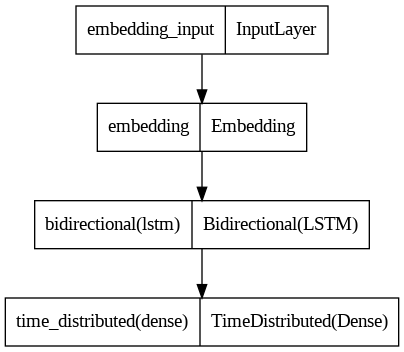
\includegraphics[scale=0.5]{img/Baseline.png}
    \caption{Baseline architecture}
    \label{fig:baseline}
\end{figure*}

\begin{figure*}[hb]
    \centering
    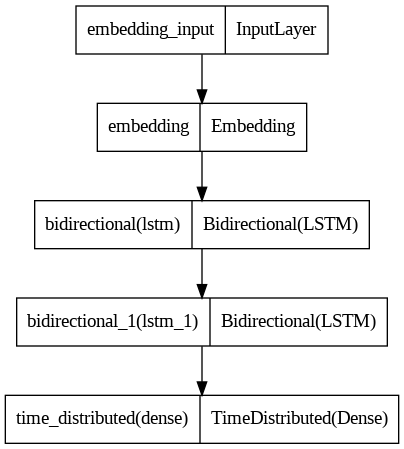
\includegraphics[scale=0.5]{img/Additional_LSTM.png}
    \caption{Additional LSTM architecture}
    \label{fig:lstm}
\end{figure*}

% \begin{figure*}[hb]
%     \centering
%     \includegraphics[width=\textwidth]{img/Additional_Dense.png}
%     \caption{Additional Dense architecture}
%     \label{fig:dense}
% \end{figure*}


\explanation{
Describe the system or systems you have implemented (architectures, pipelines, etc), and used to run your experiments. If you reuse parts of code written by others, be sure to make very clear your original contribution in terms of
\begin{itemize}
    \item architecture: is the architecture your design or did you take it from somewhere else
    \item coding: which parts of code are original or heavily adapted? adapted from existing sources? taken from external sources with minimal adaptations?
\end{itemize}
}


\section{Experimental setup and results}
\label{sec:results}

\subsection{Parameter Tuning}
Before running the experiments on the data we performed some hyperparameter tuning on each model.
During the tuning phase, we observed that the most evident changes presented themselves in the scores due to the units being used in the LSTM layer and the batch size. Generally, many units in the LSTM layer mean that the model has more capacity for complex representations. however, too many units can lead to overfitting, while a number of units between 128 and 256 can help the model memorize only the important feature of the data, which results in a more general model.
For the batch size, we used a value of 32 because a small batch improves performance and alleviates the problem of high variance in the estimated mean. Finally, with a small batch, the model is more likely to observe a more diverse range of samples in each batch, mitigating class imbalance.
The same numbers of units and batch size are then used for all the models.
\subsection{Metrics}
For the Metrics we implemented a custom function which first computes the per-sample accuracy, a binary tensor indicating if the prediction for each sample is corrected or not and then multiplies it with the weights for the corresponding true class to obtain a weighted per-sample accuracy.
After it creates a binary mask which indicates what samples to ignore in the computation of the accuracy, this mask is initialized as all ones and then updated to exclude samples with class labels specified in the arguments.
Finally, the overall weighted accuracy is computed by summing the weighted per-sample accuracy and dividing it by the number of non-ignored samples.
\subsection{Results}

\begin{table}[ht]
\caption{F1 Scores on Training Set}
\begin{tabular}{|l|l|}
\hline
                                             & \textbf{Macro F1 Scores} \\ \hline
\textbf{Baseline Model}                      & 0.7031                   \\ \hline
\textbf{GRU Model}                           & 0.6389                   \\ \hline
\textbf{Additional LSTM}                     & 0.7415                   \\ \hline
\textbf{Additional Dense}                    & 0.7002                   \\ \hline
\end{tabular}
\label{Tab:Tcr_1}
\end{table}


\begin{table}[ht]
\caption{F1 Scores on Test Set}
\begin{tabular}{|l|l|}
\hline
                                             & \textbf{Macro F1 Scores} \\ \hline
\textbf{Baseline Model}                      & 0.8345                   \\ \hline
\textbf{GRU Model}                           & 0.7446                   \\ \hline
\textbf{Additional LSTM} & 0.7808                   \\ \hline
\textbf{Additional Dense} & 0.7866                   \\ \hline
\end{tabular}
\label{Tab:Tcr_2}
\end{table}


\section{Discussion}
\label{sec:discussion}
From the results obtained, we can observe that the Baseline model performs much better on the test set compared to others, the addition of an LSTM layer helped during training, where we can see an improvement of 4\% but during evaluation if performed worse than the default model. Adding an additional Dense layer also did not improve the performance of the Baseline Model, achieving somewhat the same performance as the additional LSTM.
On the other hand, the GRU model performed the worst, achieving only 63\% during training and 74\% on the test set.


\explanation{
Here you should make your analysis of the results you obtained in your experiments. Your discussion should be structured in two parts: 
\begin{itemize}
    \item discussion of quantitative results (based on the metrics you have identified earlier; compare with baselines);
    \item error analysis: show some examples of odd/wrong/unwanted  outputs; reason about why you are getting those results, elaborate on what could/should be changed in future developments of this work.
\end{itemize}
}



\section{Conclusion}
\label{sec:conclusion}


\explanation{
In one or two paragraphs, recap your work and main results.
What did you observe? 
Did all go according to expectations? 
Was there anything surprising or worthwhile mentioning?
After that, discuss the main limitations of the solution you have implemented, and indicate promising directions for future improvement.
}



\section{Links to external resources}
\label{sec:links}
\attention{THIS SECTION IS OPTIONAL}
\explanation{
Insert here:
\begin{itemize}
    \item a link to your GitHub or any other public repo where one can find your code (only if you did not submit your code on Virtuale); 
    \item a link to your dataset (only for non-standard projects or project works).
\end{itemize}
}

\attention{DO NOT INSERT CODE IN THIS REPORT}




\bibliography{nlpreport.bib}
\end{document}